\documentclass[a4paper,11pt,uplatex]{jsarticle}


% 数式
\usepackage{amsmath,amsfonts}
\usepackage{bm}
\usepackage{physics}
% 画像
\usepackage[dvipdfmx]{graphicx}
\usepackage[dvipdfmx,colorlinks=true,linkcolor=blue]{hyperref}
\usepackage{pxjahyper}

\begin{document}


\section{Method}
\subsection{Undulator}
\subsubsection{Current operation}
\subsubsection{Position operation}

\subsection{Optical Spectrometer}
\subsubsection{grating}
\begin{itemize}
  \item Fourie Transformation
  \item spectroscopy
\end{itemize}
\subsubsection{dispersive lens and }
\begin{figure}[tb]
  \centering
  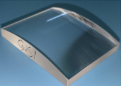
\includegraphics[width=0.8\linewidth]{image/3-lens.png}\\
  \caption{サンプルの図}
  \label{sample_image}
\end{figure}
\subsubsection{CMOS camera}











\clearpage

\begin{figure}[tb]
  \centering
  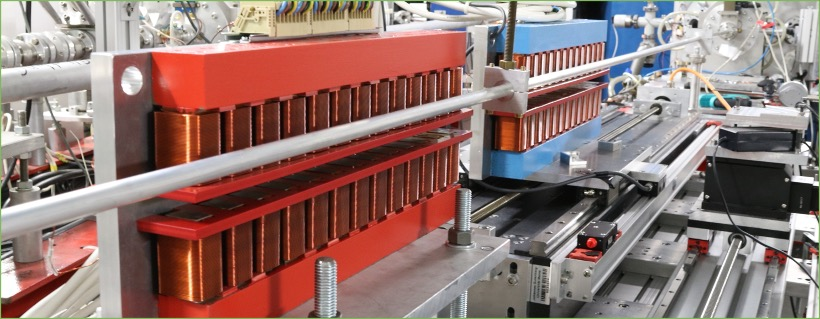
\includegraphics[width=0.8\linewidth]{image/1-1.jpg}\\
  \caption{サンプルの図}
  \label{sample_image}
\end{figure}

\begin{itemize}
  \item a
\end{itemize}
\begin{enumerate}
  \item b
\end{enumerate}

\begin{align}
\frac{1}{2} = \qty(\frac{1}{3}) + \qty{1}\Sigma
\end{align}
\end{document}